% Drawing 71/02-2 -- folder 71, batch 02, archive page 21 (PDF page 22).
% Transcription: plus bas, deux dessins sans lettres : à gauche un polygone non convexe en dents de scie, à quinze côtés environ ; à droite un petit triangle dont le côté inférieur est tracé en pointillé, avec un point au-dessus et un point au-dessous de ce côté.
% Kind: non-convex saw-tooth polygon; small triangle with one dotted side and two points. Method 2 (schematic redraw from the facsimile). Status: ok.
% Notes: Left: the saw-tooth polygon, closed, drawn through its vertices as read (fifteen of them; the long side at the lower right is slightly curved on the page and is drawn as a curve). Right: the small triangle, its lower side dotted, and the two points, one inside above that side and one below it. No letters. Agrees with the transcription's note. Redrawn 2026-11-12 (issue 128): to check again.
% Coordinates: 1 unit = 1 mm = 1/100 of the crop width (bbox in page fractions: [0.12, 0.47, 0.5, 0.64]).
% Redrawn by Claude (claude-fable-5-2), issue #128, 2026-11-12; not checked by a human; not compiled (no TeX in the session).
% Rights: reproduces part of the work -- behind RENDER_TRANSCRIPTS, never published by itself.
\documentclass[tikz,border=3pt]{standalone}
\usepackage{amsmath,amssymb}
\usetikzlibrary{patterns,arrows.meta}
\tikzset{pencil/.style={black!45}, struck/.style={black!35}, mpt/.style={circle,draw,inner sep=1.3pt}, pt/.style={circle,fill,inner sep=0.9pt}, opt/.style={circle,draw,fill=white,inner sep=1.1pt}}
\begin{document}
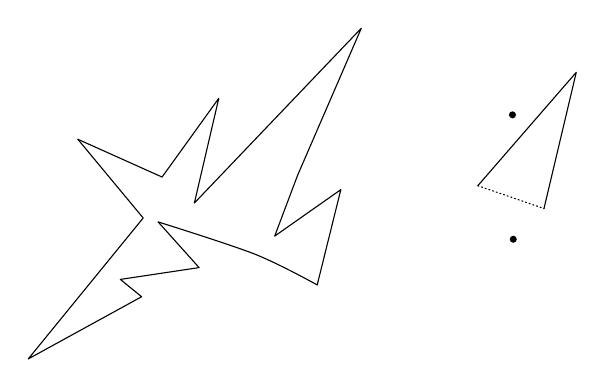
\begin{tikzpicture}[x=1mm,y=1mm,line cap=round,line join=round,font=\scriptsize]
\draw (27.5,-22.7) -- (38.2,-27.5) -- (45.4,-17.5) -- (42.3,-30.8) -- (63.5,-8.6) -- (55.4,-27.3) -- (52.5,-35) -- (60.9,-29.1) -- (57.9,-41.2);
\draw plot[smooth, tension=0.55] coordinates {(57.9,-41.2) (50,-37.3) (37.7,-33.2)};
\draw (37.7,-33.2) -- (42.9,-39) -- (32.9,-40.5) -- (35.6,-42.7) -- (21.2,-50.6) -- (35.8,-32.7) -- (27.5,-22.7);
\draw (78.3,-28.6) -- (90.8,-14.2) -- (86.7,-31.5);
\draw[densely dotted] (78.3,-28.6) -- (86.7,-31.5);
\node[pt] at (82.7,-19.6) {};
\node[pt] at (82.8,-35.4) {};
\end{tikzpicture}
\end{document}
